\chapter{Các thuật toán trên cây}

\index{cây}

Một \key{cây} là một đồ thị liên thông, không có chu trình
bao gồm $n$ nút và $n-1$ cạnh.
Việc loại bỏ bất kỳ cạnh nào khỏi cây sẽ chia nó
thành hai thành phần,
và việc thêm bất kỳ cạnh nào vào cây sẽ tạo ra một chu trình.
Hơn nữa, luôn có một đường đi duy nhất giữa bất kỳ
hai nút nào của một cây.

Ví dụ, cây sau bao gồm 8 nút và 7 cạnh:
\begin{center}
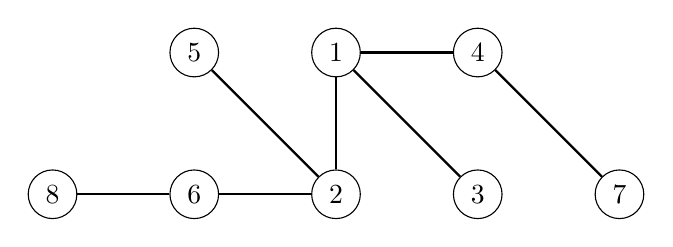
\begin{tikzpicture}[scale=0.9]
\node[draw, circle] (1) at (0,3) {$1$};
\node[draw, circle] (2) at (2,3) {$4$};
\node[draw, circle] (3) at (0,1) {$2$};
\node[draw, circle] (4) at (2,1) {$3$};
\node[draw, circle] (5) at (4,1) {$7$};
\node[draw, circle] (6) at (-2,3) {$5$};
\node[draw, circle] (7) at (-2,1) {$6$};
\node[draw, circle] (8) at (-4,1) {$8$};
\path[draw,thick,-] (1) -- (2);
\path[draw,thick,-] (1) -- (3);
\path[draw,thick,-] (1) -- (4);
\path[draw,thick,-] (2) -- (5);
\path[draw,thick,-] (3) -- (6);
\path[draw,thick,-] (3) -- (7);
\path[draw,thick,-] (7) -- (8);
\end{tikzpicture}
\end{center}

\index{lá}

Các \key{lá} của một cây là các nút
có bậc 1, tức là chỉ có một hàng xóm.
Ví dụ, các lá của cây trên
là các nút 3, 5, 7 và 8.

\index{gốc}
\index{cây có gốc}

Trong một cây \key{có gốc}, một trong các nút
được chỉ định làm \key{gốc} của cây,
và tất cả các nút khác được
đặt bên dưới gốc.
Ví dụ, trong cây sau,
nút 1 là nút gốc.

\begin{center}
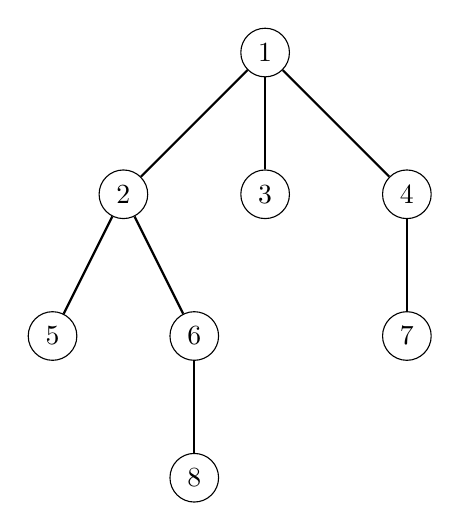
\begin{tikzpicture}[scale=0.9]
\node[draw, circle] (1) at (0,3) {$1$};
\node[draw, circle] (4) at (2,1) {$4$};
\node[draw, circle] (2) at (-2,1) {$2$};
\node[draw, circle] (3) at (0,1) {$3$};
\node[draw, circle] (7) at (2,-1) {$7$};
\node[draw, circle] (5) at (-3,-1) {$5$};
\node[draw, circle] (6) at (-1,-1) {$6$};
\node[draw, circle] (8) at (-1,-3) {$8$};
\path[draw,thick,-] (1) -- (2);
\path[draw,thick,-] (1) -- (3);
\path[draw,thick,-] (1) -- (4);
\path[draw,thick,-] (2) -- (5);
\path[draw,thick,-] (2) -- (6);
\path[draw,thick,-] (4) -- (7);
\path[draw,thick,-] (6) -- (8);
\end{tikzpicture}
\end{center}
\index{con}
\index{cha}

Trong một cây có gốc, các \key{con} của một nút
là các hàng xóm dưới của nó, và \key{cha} của một nút
là hàng xóm trên của nó.
Mỗi nút có đúng một cha,
ngoại trừ gốc không có cha.
Ví dụ, trong cây trên,
các con của nút 2 là các nút 5 và 6,
và cha của nó là nút 1.

\index{cây con}

Cấu trúc của một cây có gốc là \emph{đệ quy}:
mỗi nút của cây hoạt động như gốc của một \key{cây con}
chứa chính nút đó và tất cả các nút
nằm trong các cây con của các con của nó.
Ví dụ, trong cây trên, cây con của nút 2
bao gồm các nút 2, 5, 6 và 8:
\begin{center}
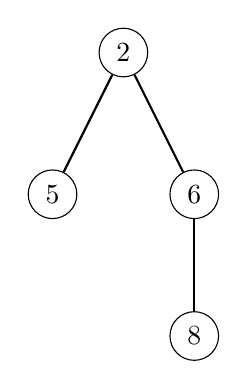
\begin{tikzpicture}[scale=0.9]
\node[draw, circle] (2) at (-2,1) {$2$};
\node[draw, circle] (5) at (-3,-1) {$5$};
\node[draw, circle] (6) at (-1,-1) {$6$};
\node[draw, circle] (8) at (-1,-3) {$8$};
\path[draw,thick,-] (2) -- (5);
\path[draw,thick,-] (2) -- (6);
\path[draw,thick,-] (6) -- (8);
\end{tikzpicture}
\end{center}

\section{Duyệt cây}

Các thuật toán duyệt đồ thị tổng quát
có thể được sử dụng để duyệt các nút của một cây.
Tuy nhiên, việc duyệt một cây dễ cài đặt hơn
so với một đồ thị tổng quát, bởi vì
không có chu trình trong cây và không thể
đến một nút từ nhiều hướng.

Cách điển hình để duyệt một cây là bắt đầu
một tìm kiếm theo chiều sâu tại một nút tùy ý.
Hàm đệ quy sau có thể được sử dụng:

\begin{lstlisting}
void dfs(int s, int e) {
    // xu ly nut s
    for (auto u : adj[s]) {
        if (u != e) dfs(u, s);
    }
}
\end{lstlisting}

Hàm được cung cấp hai tham số: nút hiện tại $s$
và nút trước đó $e$.
Mục đích của tham số $e$ là để đảm bảo
rằng tìm kiếm chỉ di chuyển đến các nút
chưa được thăm.

Lệnh gọi hàm sau bắt đầu tìm kiếm
tại nút $x$:

\begin{lstlisting}
dfs(x, 0);
\end{lstlisting}

Trong lệnh gọi đầu tiên $e=0$, bởi vì không có
nút trước đó, và được phép
tiến đến bất kỳ hướng nào trong cây.

\subsubsection{Quy hoạch động}

Quy hoạch động có thể được sử dụng để tính toán
một số thông tin trong quá trình duyệt cây.
Sử dụng quy hoạch động, chúng ta có thể, ví dụ,
tính toán trong thời gian $O(n)$ cho mỗi nút của một cây có gốc
số lượng nút trong cây con của nó
hoặc độ dài của đường đi dài nhất từ nút đó
đến một lá.

Ví dụ, chúng ta hãy tính toán cho mỗi nút $s$
một giá trị $\texttt{count}[s]$: số lượng nút trong cây con của nó.
Cây con chứa chính nút đó và
tất cả các nút trong các cây con của các con của nó,
vì vậy chúng ta có thể tính toán số lượng nút
một cách đệ quy bằng cách sử dụng đoạn mã sau:

\begin{lstlisting}
void dfs(int s, int e) {
    count[s] = 1;
    for (auto u : adj[s]) {
        if (u == e) continue;
        dfs(u, s);
        count[s] += count[u];
    }
}
\end{lstlisting}

\section{Đường kính}

\index{đường kính}

\key{Đường kính} của một cây
là độ dài tối đa của một đường đi giữa hai nút.
Ví dụ, hãy xem xét cây sau:
\begin{center}
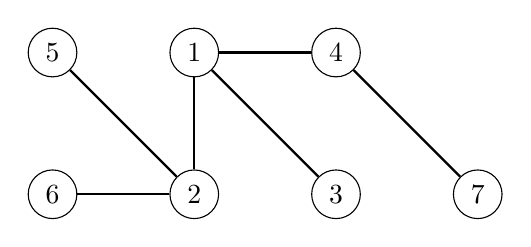
\begin{tikzpicture}[scale=0.9]
\node[draw, circle] (1) at (0,3) {$1$};
\node[draw, circle] (2) at (2,3) {$4$};
\node[draw, circle] (3) at (0,1) {$2$};
\node[draw, circle] (4) at (2,1) {$3$};
\node[draw, circle] (5) at (4,1) {$7$};
\node[draw, circle] (6) at (-2,3) {$5$};
\node[draw, circle] (7) at (-2,1) {$6$};
\path[draw,thick,-] (1) -- (2);
\path[draw,thick,-] (1) -- (3);
\path[draw,thick,-] (1) -- (4);
\path[draw,thick,-] (2) -- (5);
\path[draw,thick,-] (3) -- (6);
\path[draw,thick,-] (3) -- (7);
\end{tikzpicture}
\end{center}
Đường kính của cây này là 4,
tương ứng với đường đi sau:
\begin{center}
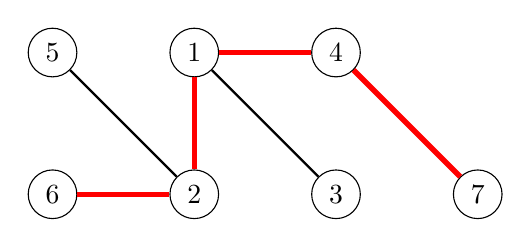
\begin{tikzpicture}[scale=0.9]
\node[draw, circle] (1) at (0,3) {$1$};
\node[draw, circle] (2) at (2,3) {$4$};
\node[draw, circle] (3) at (0,1) {$2$};
\node[draw, circle] (4) at (2,1) {$3$};
\node[draw, circle] (5) at (4,1) {$7$};
\node[draw, circle] (6) at (-2,3) {$5$};
\node[draw, circle] (7) at (-2,1) {$6$};
\path[draw,thick,-] (1) -- (2);
\path[draw,thick,-] (1) -- (3);
\path[draw,thick,-] (1) -- (4);
\path[draw,thick,-] (2) -- (5);
\path[draw,thick,-] (3) -- (6);
\path[draw,thick,-] (3) -- (7);

\path[draw,thick,-,color=red,line width=2pt] (7) -- (3);
\path[draw,thick,-,color=red,line width=2pt] (3) -- (1);
\path[draw,thick,-,color=red,line width=2pt] (1) -- (2);
\path[draw,thick,-,color=red,line width=2pt] (2) -- (5);
\end{tikzpicture}
\end{center}
Lưu ý rằng có thể có nhiều đường đi có độ dài tối đa.
Trong đường đi trên, chúng ta có thể thay thế nút 6 bằng nút 5
để có được một đường đi khác có độ dài 4.

Tiếp theo chúng ta sẽ thảo luận về hai thuật toán thời gian $O(n)$
để tính đường kính của một cây.
Thuật toán đầu tiên dựa trên quy hoạch động,
và thuật toán thứ hai sử dụng hai lần tìm kiếm theo chiều sâu.

\subsubsection{Thuật toán 1}

Một cách tiếp cận chung cho nhiều bài toán trên cây
là trước tiên gốc hóa cây một cách tùy ý.
Sau đó, chúng ta có thể cố gắng giải quyết bài toán
một cách riêng biệt cho mỗi cây con.
Thuật toán đầu tiên của chúng ta để tính đường kính
dựa trên ý tưởng này.

Một quan sát quan trọng là mọi đường đi
trong một cây có gốc đều có một \emph{điểm cao nhất}:
nút cao nhất thuộc về đường đi.
Do đó, chúng ta có thể tính toán cho mỗi nút độ dài
của đường đi dài nhất có điểm cao nhất là nút đó.
Một trong những đường đi đó tương ứng với đường kính của cây.

Ví dụ, trong cây sau,
nút 1 là điểm cao nhất trên đường đi
tương ứng với đường kính:
\begin{center}
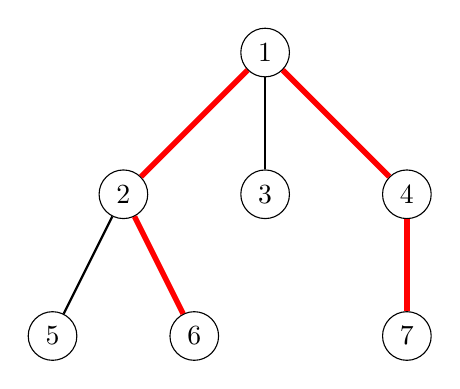
\begin{tikzpicture}[scale=0.9]
\node[draw, circle] (1) at (0,3) {$1$};
\node[draw, circle] (2) at (2,1) {$4$};
\node[draw, circle] (3) at (-2,1) {$2$};
\node[draw, circle] (4) at (0,1) {$3$};
\node[draw, circle] (5) at (2,-1) {$7$};
\node[draw, circle] (6) at (-3,-1) {$5$};
\node[draw, circle] (7) at (-1,-1) {$6$};
\path[draw,thick,-] (1) -- (2);
\path[draw,thick,-] (1) -- (3);
\path[draw,thick,-] (1) -- (4);
\path[draw,thick,-] (2) -- (5);
\path[draw,thick,-] (3) -- (6);
\path[draw,thick,-] (3) -- (7);

\path[draw,thick,-,color=red,line width=2pt] (7) -- (3);
\path[draw,thick,-,color=red,line width=2pt] (3) -- (1);
\path[draw,thick,-,color=red,line width=2pt] (1) -- (2);
\path[draw,thick,-,color=red,line width=2pt] (2) -- (5);
\end{tikzpicture}
\end{center}

Chúng ta tính toán cho mỗi nút $x$ hai giá trị:
\begin{itemize}
\item $\texttt{toLeaf}(x)$: độ dài tối đa của một đường đi từ $x$ đến bất kỳ lá nào
\item $\texttt{maxLength}(x)$: độ dài tối đa của một đường đi
có điểm cao nhất là $x$
\end{itemize}
Ví dụ, trong cây trên,
$\texttt{toLeaf}(1)=2$, vì có một đường đi
$1 \rightarrow 2 \rightarrow 6$,
và $\texttt{maxLength}(1)=4$,
vì có một đường đi
$6 \rightarrow 2 \rightarrow 1 \rightarrow 4 \rightarrow 7$.
Trong trường hợp này, $\texttt{maxLength}(1)$ bằng với đường kính.

Quy hoạch động có thể được sử dụng để tính toán các giá trị trên
cho tất cả các nút trong thời gian $O(n)$.
Đầu tiên, để tính $\texttt{toLeaf}(x)$,
chúng ta đi qua các con của $x$,
chọn một con $c$ có $\texttt{toLeaf}(c)$ lớn nhất
và cộng một vào giá trị này.
Sau đó, để tính $\texttt{maxLength}(x)$,
chúng ta chọn hai con riêng biệt $a$ và $b$
sao cho tổng $\texttt{toLeaf}(a)+\texttt{toLeaf}(b)$
là lớn nhất và cộng hai vào tổng này.

\subsubsection{Thuật toán 2}

Một cách hiệu quả khác để tính đường kính
của một cây là dựa trên hai lần tìm kiếm theo chiều sâu.
Đầu tiên, chúng ta chọn một nút tùy ý $a$ trong cây
và tìm nút xa nhất $b$ từ $a$.
Sau đó, chúng ta tìm nút xa nhất $c$ từ $b$.
Đường kính của cây là khoảng cách giữa $b$ và $c$.

Trong đồ thị sau, $a$, $b$ và $c$ có thể là:
\begin{center}
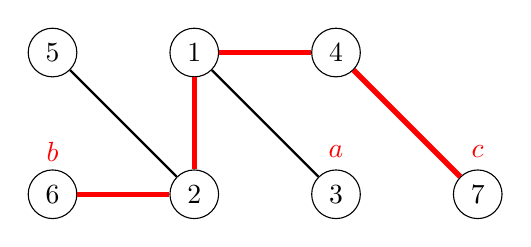
\begin{tikzpicture}[scale=0.9]
\node[draw, circle] (1) at (0,3) {$1$};
\node[draw, circle] (2) at (2,3) {$4$};
\node[draw, circle] (3) at (0,1) {$2$};
\node[draw, circle] (4) at (2,1) {$3$};
\node[draw, circle] (5) at (4,1) {$7$};
\node[draw, circle] (6) at (-2,3) {$5$};
\node[draw, circle] (7) at (-2,1) {$6$};
\path[draw,thick,-] (1) -- (2);
\path[draw,thick,-] (1) -- (3);
\path[draw,thick,-] (1) -- (4);
\path[draw,thick,-] (2) -- (5);
\path[draw,thick,-] (3) -- (6);
\path[draw,thick,-] (3) -- (7);
\node[color=red] at (2,1.6) {$a$};
\node[color=red] at (-2,1.6) {$b$};
\node[color=red] at (4,1.6) {$c$};

\path[draw,thick,-,color=red,line width=2pt] (7) -- (3);
\path[draw,thick,-,color=red,line width=2pt] (3) -- (1);
\path[draw,thick,-,color=red,line width=2pt] (1) -- (2);
\path[draw,thick,-,color=red,line width=2pt] (2) -- (5);
\end{tikzpicture}
\end{center}

Đây là một phương pháp thanh lịch, nhưng tại sao nó hoạt động?

Sẽ hữu ích nếu vẽ cây theo một cách khác để
đường đi tương ứng với đường kính
là nằm ngang, và tất cả các nút khác
treo trên nó:
\begin{center}
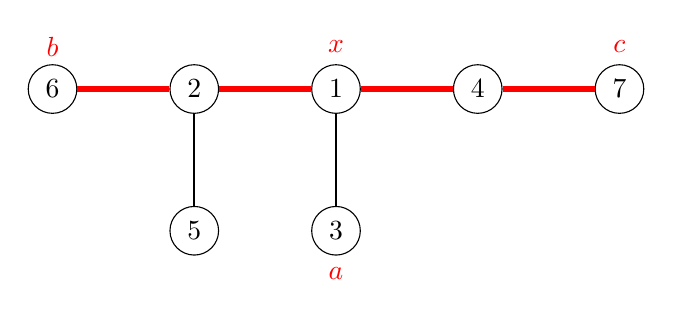
\begin{tikzpicture}[scale=0.9]
\node[draw, circle] (1) at (2,1) {$1$};
\node[draw, circle] (2) at (4,1) {$4$};
\node[draw, circle] (3) at (0,1) {$2$};
\node[draw, circle] (4) at (2,-1) {$3$};
\node[draw, circle] (5) at (6,1) {$7$};
\node[draw, circle] (6) at (0,-1) {$5$};
\node[draw, circle] (7) at (-2,1) {$6$};
\path[draw,thick,-] (1) -- (2);
\path[draw,thick,-] (1) -- (3);
\path[draw,thick,-] (1) -- (4);
\path[draw,thick,-] (2) -- (5);
\path[draw,thick,-] (3) -- (6);
\path[draw,thick,-] (3) -- (7);
\node[color=red] at (2,-1.6) {$a$};
\node[color=red] at (-2,1.6) {$b$};
\node[color=red] at (6,1.6) {$c$};
\node[color=red] at (2,1.6) {$x$};

\path[draw,thick,-,color=red,line width=2pt] (7) -- (3);
\path[draw,thick,-,color=red,line width=2pt] (3) -- (1);
\path[draw,thick,-,color=red,line width=2pt] (1) -- (2);
\path[draw,thick,-,color=red,line width=2pt] (2) -- (5);
\end{tikzpicture}
\end{center}

Nút $x$ chỉ ra nơi mà đường đi
từ nút $a$ nối với đường đi tương ứng
với đường kính.
Nút xa nhất từ $a$
là nút $b$, nút $c$ hoặc một số nút khác
ít nhất cũng xa như từ nút $x$.
Do đó, nút này luôn là một lựa chọn hợp lệ cho
một điểm cuối của một đường đi tương ứng với đường kính.

\section{Tất cả các đường đi dài nhất}

Bài toán tiếp theo của chúng ta là tính toán cho mọi nút
trong cây độ dài tối đa của một đường đi
bắt đầu tại nút đó.
Điều này có thể được xem như một sự tổng quát hóa của
bài toán đường kính cây, bởi vì lớn nhất trong số các
độ dài đó bằng với đường kính của cây.
Bài toán này cũng có thể được giải quyết trong thời gian $O(n)$.

Ví dụ, hãy xem xét cây sau:
\begin{center}
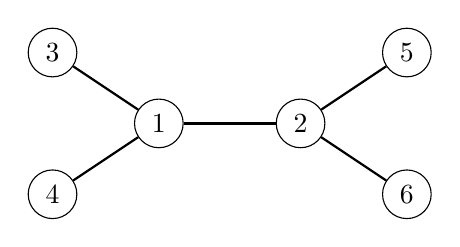
\begin{tikzpicture}[scale=0.9]
\node[draw, circle] (1) at (0,0) {$1$};
\node[draw, circle] (2) at (-1.5,-1) {$4$};
\node[draw, circle] (3) at (2,0) {$2$};
\node[draw, circle] (4) at (-1.5,1) {$3$};
\node[draw, circle] (6) at (3.5,-1) {$6$};
\node[draw, circle] (7) at (3.5,1) {$5$};
\path[draw,thick,-] (1) -- (2);
\path[draw,thick,-] (1) -- (3);
\path[draw,thick,-] (1) -- (4);
\path[draw,thick,-] (3) -- (6);
\path[draw,thick,-] (3) -- (7);
\end{tikzpicture}
\end{center}

Gọi $\texttt{maxLength}(x)$ là độ dài tối đa
của một đường đi bắt đầu tại nút $x$.
Ví dụ, trong cây trên,
$\texttt{maxLength}(4)=3$, vì có
một đường đi $4 \rightarrow 1 \rightarrow 2 \rightarrow 6$.
Đây là một bảng đầy đủ các giá trị:
\begin{center}
\begin{tabular}{l|lllllll}
nút $x$ & 1 & 2 & 3 & 4 & 5 & 6 \\
$\texttt{maxLength}(x)$ & 2 & 2 & 3 & 3 & 3 & 3 \\
\end{tabular}
\end{center}

Cũng trong bài toán này, một điểm khởi đầu tốt
để giải quyết bài toán là gốc hóa cây một cách tùy ý:
\begin{center}
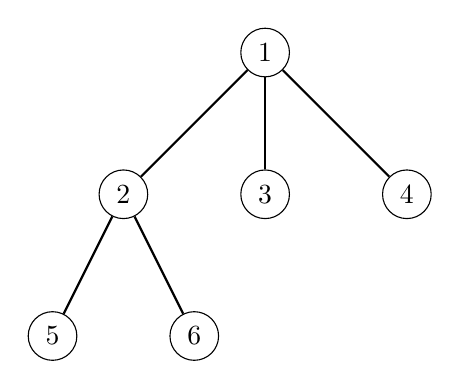
\begin{tikzpicture}[scale=0.9]
\node[draw, circle] (1) at (0,3) {$1$};
\node[draw, circle] (2) at (2,1) {$4$};
\node[draw, circle] (3) at (-2,1) {$2$};
\node[draw, circle] (4) at (0,1) {$3$};
\node[draw, circle] (6) at (-3,-1) {$5$};
\node[draw, circle] (7) at (-1,-1) {$6$};
\path[draw,thick,-] (1) -- (2);
\path[draw,thick,-] (1) -- (3);
\path[draw,thick,-] (1) -- (4);
\path[draw,thick,-] (3) -- (6);
\path[draw,thick,-] (3) -- (7);
\end{tikzpicture}
\end{center}

Phần đầu tiên của bài toán là tính toán cho mọi nút $x$
độ dài tối đa của một đường đi đi qua một con của $x$.
Ví dụ, đường đi dài nhất từ nút 1
đi qua con của nó là 2:
\begin{center}
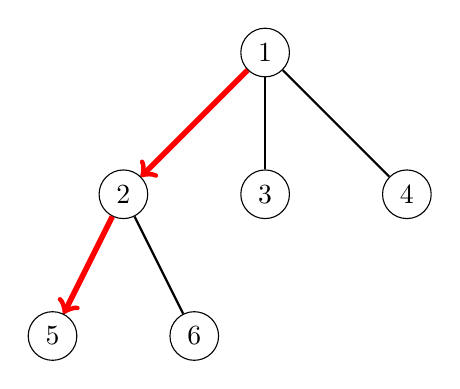
\begin{tikzpicture}[scale=0.9]
\node[draw, circle] (1) at (0,3) {$1$};
\node[draw, circle] (2) at (2,1) {$4$};
\node[draw, circle] (3) at (-2,1) {$2$};
\node[draw, circle] (4) at (0,1) {$3$};
\node[draw, circle] (6) at (-3,-1) {$5$};
\node[draw, circle] (7) at (-1,-1) {$6$};
\path[draw,thick,-] (1) -- (2);
\path[draw,thick,-] (1) -- (3);
\path[draw,thick,-] (1) -- (4);
\path[draw,thick,-] (3) -- (6);
\path[draw,thick,-] (3) -- (7);

\path[draw,thick,->,color=red,line width=2pt] (1) -- (3);
\path[draw,thick,->,color=red,line width=2pt] (3) -- (6);
\end{tikzpicture}
\end{center}
Phần này dễ giải quyết trong thời gian $O(n)$, vì chúng ta có thể sử dụng
quy hoạch động như chúng ta đã làm trước đây.

Sau đó, phần thứ hai của bài toán là tính toán
cho mọi nút $x$ độ dài tối đa của một đường đi
đi qua cha của nó là $p$.
Ví dụ, đường đi dài nhất
từ nút 3 đi qua cha của nó là 1:
\begin{center}
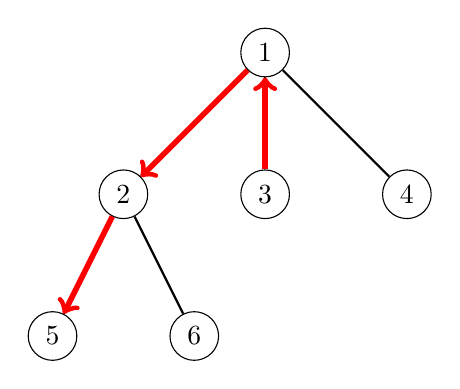
\begin{tikzpicture}[scale=0.9]
\node[draw, circle] (1) at (0,3) {$1$};
\node[draw, circle] (2) at (2,1) {$4$};
\node[draw, circle] (3) at (-2,1) {$2$};
\node[draw, circle] (4) at (0,1) {$3$};
\node[draw, circle] (6) at (-3,-1) {$5$};
\node[draw, circle] (7) at (-1,-1) {$6$};
\path[draw,thick,-] (1) -- (2);
\path[draw,thick,-] (1) -- (3);
\path[draw,thick,-] (1) -- (4);
\path[draw,thick,-] (3) -- (6);
\path[draw,thick,-] (3) -- (7);

\path[draw,thick,->,color=red,line width=2pt] (4) -- (1);
\path[draw,thick,->,color=red,line width=2pt] (1) -- (3);
\path[draw,thick,->,color=red,line width=2pt] (3) -- (6);
\end{tikzpicture}
\end{center}

Thoạt nhìn, có vẻ như chúng ta nên chọn
đường đi dài nhất từ $p$.
Tuy nhiên, điều này \emph{không} phải lúc nào cũng hoạt động,
bởi vì đường đi dài nhất từ $p$
có thể đi qua $x$.
Đây là một ví dụ về tình huống này:
\begin{center}
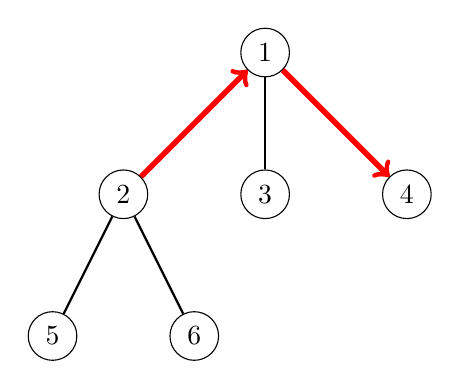
\begin{tikzpicture}[scale=0.9]
\node[draw, circle] (1) at (0,3) {$1$};
\node[draw, circle] (2) at (2,1) {$4$};
\node[draw, circle] (3) at (-2,1) {$2$};
\node[draw, circle] (4) at (0,1) {$3$};
\node[draw, circle] (6) at (-3,-1) {$5$};
\node[draw, circle] (7) at (-1,-1) {$6$};
\path[draw,thick,-] (1) -- (2);
\path[draw,thick,-] (1) -- (3);
\path[draw,thick,-] (1) -- (4);
\path[draw,thick,-] (3) -- (6);
\path[draw,thick,-] (3) -- (7);

\path[draw,thick,->,color=red,line width=2pt] (3) -- (1);
\path[draw,thick,->,color=red,line width=2pt] (1) -- (2);
\end{tikzpicture}
\end{center}

Tuy nhiên, chúng ta có thể giải quyết phần thứ hai trong
thời gian $O(n)$ bằng cách lưu trữ \emph{hai} độ dài tối đa
cho mỗi nút $x$:
\begin{itemize}
\item $\texttt{maxLength}_1(x)$:
độ dài tối đa của một đường đi từ $x$
\item $\texttt{maxLength}_2(x)$
độ dài tối đa của một đường đi từ $x$
theo một hướng khác với đường đi đầu tiên
\end{itemize}
Ví dụ, trong đồ thị trên,
$\texttt{maxLength}_1(1)=2$
sử dụng đường đi $1 \rightarrow 2 \rightarrow 5$,
và $\texttt{maxLength}_2(1)=1$
sử dụng đường đi $1 \rightarrow 3$.

Cuối cùng, nếu đường đi tương ứng với
$\texttt{maxLength}_1(p)$ đi qua $x$,
chúng ta kết luận rằng độ dài tối đa là
$\texttt{maxLength}_2(p)+1$,
và ngược lại, độ dài tối đa là
$\texttt{maxLength}_1(p)+1$.


\section{Cây nhị phân}

\index{cây nhị phân}

\begin{samepage}
Một \key{cây nhị phân} là một cây có gốc
trong đó mỗi nút có một cây con trái và một cây con phải.
Có thể một cây con của một nút là rỗng.
Do đó, mọi nút trong một cây nhị phân có
không, một hoặc hai con.

Ví dụ, cây sau là một cây nhị phân:
\begin{center}
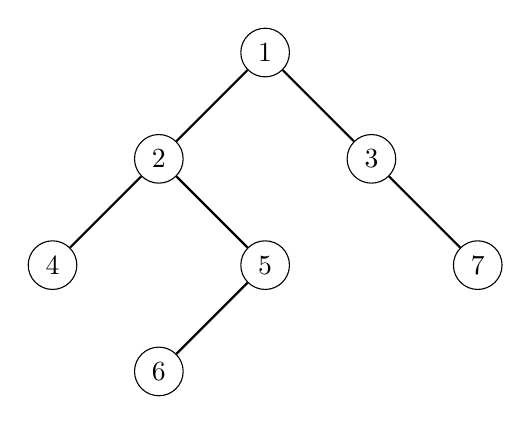
\begin{tikzpicture}[scale=0.9]
\node[draw, circle] (1) at (0,0) {$1$};
\node[draw, circle] (2) at (-1.5,-1.5) {$2$};
\node[draw, circle] (3) at (1.5,-1.5) {$3$};
\node[draw, circle] (4) at (-3,-3) {$4$};
\node[draw, circle] (5) at (0,-3) {$5$};
\node[draw, circle] (6) at (-1.5,-4.5) {$6$};
\node[draw, circle] (7) at (3,-3) {$7$};

\path[draw,thick,-] (1) -- (2);
\path[draw,thick,-] (1) -- (3);
\path[draw,thick,-] (2) -- (4);
\path[draw,thick,-] (2) -- (5);
\path[draw,thick,-] (5) -- (6);
\path[draw,thick,-] (3) -- (7);
\end{tikzpicture}
\end{center}
\end{samepage}

\index{tiền thứ tự}
\index{trung thứ tự}
\index{hậu thứ tự}

Các nút của một cây nhị phân có ba thứ tự
tự nhiên tương ứng với các cách khác nhau để
duyệt cây một cách đệ quy:

\begin{itemize}
\item \key{tiền thứ tự}: đầu tiên xử lý gốc,
sau đó duyệt cây con trái, sau đó duyệt cây con phải
\item \key{trung thứ tự}: đầu tiên duyệt cây con trái,
sau đó xử lý gốc, sau đó duyệt cây con phải
\item \key{hậu thứ tự}: đầu tiên duyệt cây con trái,
sau đó duyệt cây con phải, sau đó xử lý gốc
\end{itemize}

Đối với cây trên, các nút theo
tiền thứ tự là
$[1,2,4,5,6,3,7]$,
theo trung thứ tự là $[4,2,6,5,1,3,7]$
và theo hậu thứ tự là $[4,6,5,2,7,3,1]$.

Nếu chúng ta biết thứ tự tiền thứ tự và trung thứ tự
của một cây, chúng ta có thể tái tạo lại cấu trúc chính xác của cây.
Ví dụ, cây trên là cây duy nhất có thể có
với thứ tự tiền thứ tự là $[1,2,4,5,6,3,7]$ và
thứ tự trung thứ tự là $[4,2,6,5,1,3,7]$.
Tương tự, thứ tự hậu thứ tự và trung thứ tự
cũng xác định cấu trúc của một cây.

Tuy nhiên, tình hình sẽ khác nếu chúng ta chỉ biết
thứ tự tiền thứ tự và hậu thứ tự của một cây.
Trong trường hợp này, có thể có nhiều hơn một cây
khớp với các thứ tự.
Ví dụ, trong cả hai cây
\begin{center}
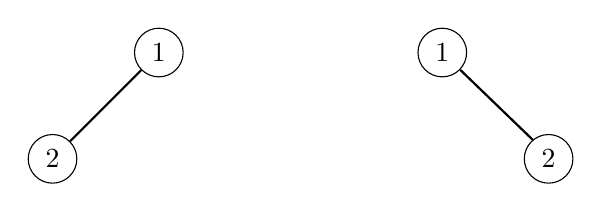
\begin{tikzpicture}[scale=0.9]
\node[draw, circle] (1) at (0,0) {$1$};
\node[draw, circle] (2) at (-1.5,-1.5) {$2$};
\path[draw,thick,-] (1) -- (2);

\node[draw, circle] (1b) at (0+4,0) {$1$};
\node[draw, circle] (2b) at (1.5+4,-1.5) {$2$};
\path[draw,thick,-] (1b) -- (2b);
\end{tikzpicture}
\end{center}
thứ tự tiền thứ tự là $[1,2]$ và thứ tự hậu thứ tự là $[2,1]$,
nhưng cấu trúc của các cây là khác nhau.

